\chapter{Исследовательский раздел}

Характеристики компьютера, на котором было проведено тестирование разработанного ПО: операционная система Debian Bookworm, версия ядра Linux 6.1.31.

На рисунке \ref{img:test} представлен пример отображения на дисплее информации о потребляемой процессом containerd виртуальной памяти.

\begin{table}[h!]
  \centering
  \begin{tabular}{p{1\linewidth}}
    \centering
    
\includegraphics[width=0.8\linewidth]{./images/test.pdf}
    \captionof{figure}{Пример отображения на дисплее информации о потребляемой процессом containerd виртуальной памяти}
    \label{img:test}
  \end{tabular}
\end{table}

На рисунках \ref{img:sfu}~--~\ref{img:mod} представлен пример отображения в системе специального файла устройства для разработанного драйвера и модуля ядра соответственно.

\begin{table}[h!]
  \centering
  \begin{tabular}{p{1\linewidth}}
    \centering
    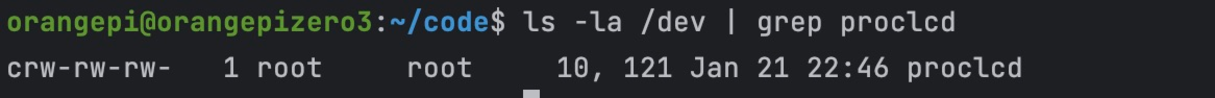
\includegraphics[width=0.9\linewidth]{./images/sfu.pdf}
    \captionof{figure}{Пример отображения в системе специального файла устройства для разработанного драйвера}
    \label{img:sfu}
  \end{tabular}
\end{table}

\begin{table}[h!]
  \centering
  \begin{tabular}{p{1\linewidth}}
    \centering
    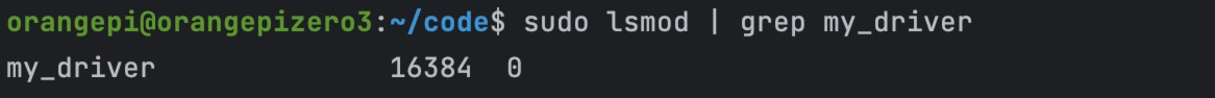
\includegraphics[width=0.9\linewidth]{./images/mod.pdf}
    \captionof{figure}{Пример отображения в системе модуля ядра}
    \label{img:mod}
  \end{tabular}
\end{table}

На рисунках \ref{img:out_init}~--~\ref{img:out_print} представлен пример логов разработанного модуля ядра при инициализации и в процессе вывода данных на дисплей соответственно.

\begin{table}[h!]
  \centering
  \begin{tabular}{p{1\linewidth}}
    \centering
    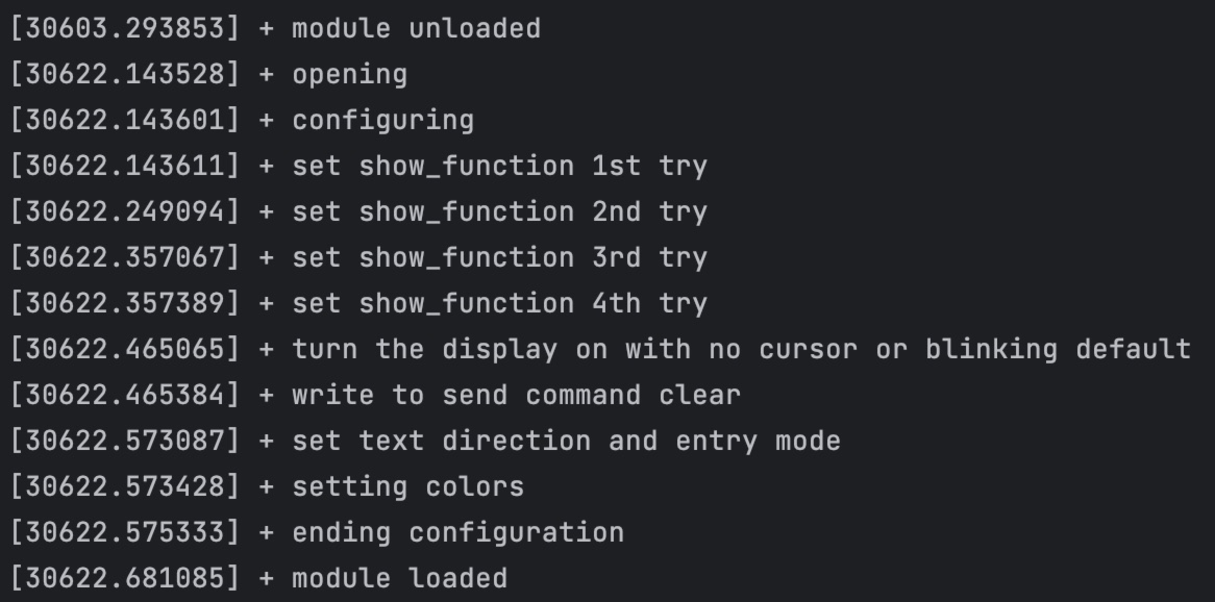
\includegraphics[width=0.8\linewidth]{./images/out_init.pdf}
    \captionof{figure}{Пример логов разработанного модуля ядра при инициализации}
    \label{img:out_init}
  \end{tabular}
\end{table}

\begin{table}[h!]
  \centering
  \begin{tabular}{p{1\linewidth}}
    \centering
    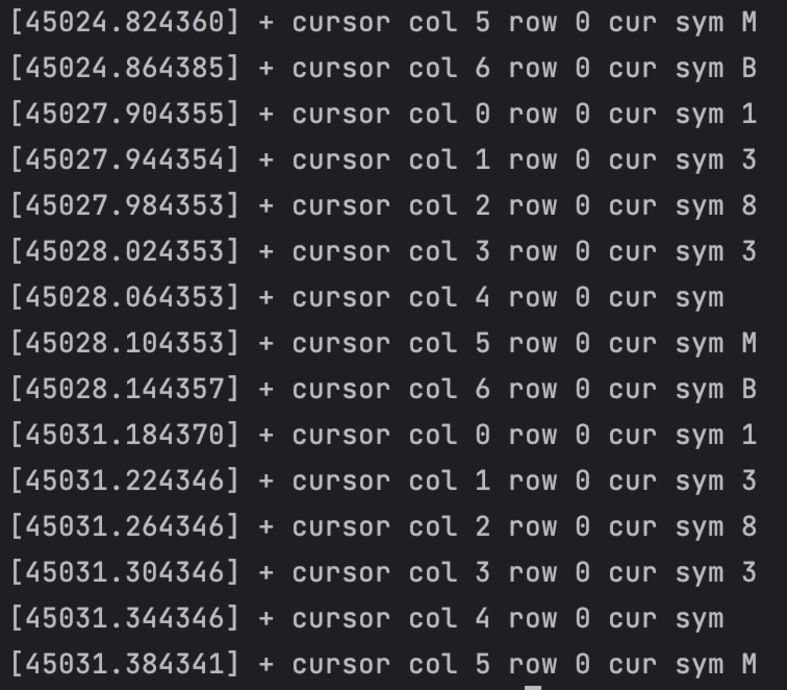
\includegraphics[width=0.6\linewidth]{./images/out_print.pdf}
    \captionof{figure}{Пример логов разработанного модуля ядра в процессе вывода данных на дисплей}
    \label{img:out_print}
  \end{tabular}
\end{table}

\newpage
На рисунке \ref{img:if} представлен интерфейс клиентской части приложения.
\newpage

\begin{table}[h!]
  \centering
  \begin{tabular}{p{1\linewidth}}
    \centering
    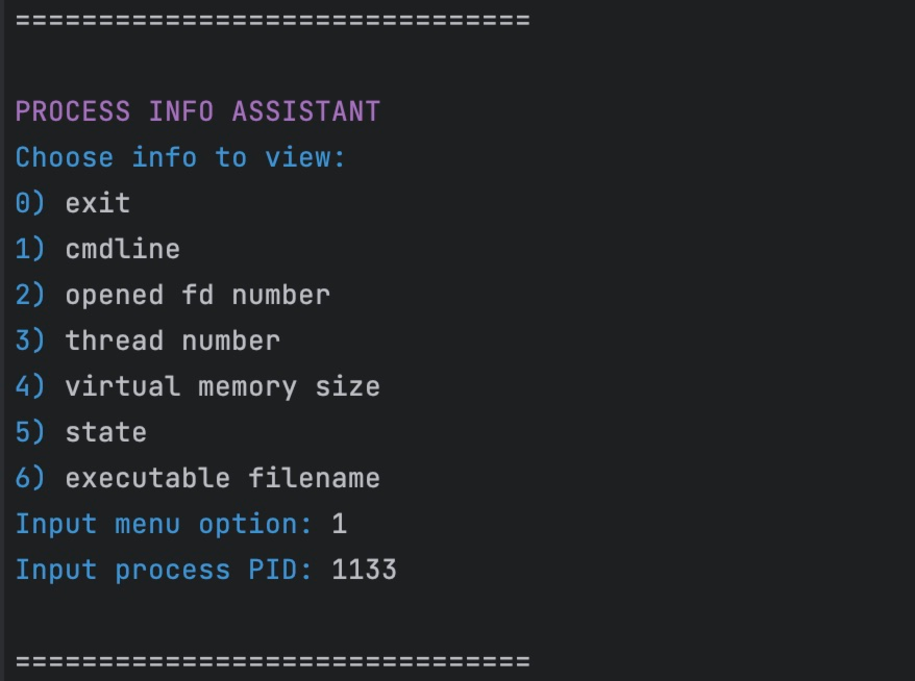
\includegraphics[width=0.7\linewidth]{./images/if.pdf}
    \captionof{figure}{Интерфейс клиентской части приложения}
    \label{img:if}
  \end{tabular}
\end{table}

\section*{Вывод}
Был представлен пример отображения информации о конкретном процессе на символьном дисплее. Также, были приведены примеры отображения в системе специального файла устройства, отображение модуля ядра, пример отладочного вывода разработанного модуля и вид пользовательского интерфейса.

\newpage
